\documentclass{article}

\usepackage[utf8]{inputenc}
\usepackage{natbib} 
\usepackage{graphicx}
\usepackage{polski}
\usepackage{tikz}
\usepackage{listings}
\usepackage{xcolor}

\definecolor{codegreen}{rgb}{0,0.6,0}
\definecolor{codegray}{rgb}{0.5,0.5,0.5}
\definecolor{codepurple}{rgb}{0.58,0,0.82}
\definecolor{backcolour}{rgb}{0.95,0.95,0.92}

\lstdefinestyle{mystyle}{
    backgroundcolor=\color{backcolour},   
    commentstyle=\color{codegreen},
    keywordstyle=\color{teal},
    numberstyle=\tiny\color{codegray},
    stringstyle=\color{codepurple},
    basicstyle=\ttfamily\footnotesize,
    breakatwhitespace=false,         
    breaklines=true,                 
    captionpos=b,                    
    keepspaces=true,                 
    numbers=left,                    
    numbersep=5pt,                  
    showspaces=false,                
    showstringspaces=false,
    showtabs=false,                  
    tabsize=2
}

\lstset{style=mystyle}

\usepackage{hyperref}
\hypersetup{
    colorlinks=true,
    linkcolor=black,
    filecolor=black,      
    urlcolor=blue,
}



\title{Interfejsy i Multimedia w Technice Gr.22}
\author{
    Grzegorz Kupczyk
    \and
    Adam Bernard
    \and
    Jarosław Bartkowski
}
\date{Kwiecień 2021}

\begin{document}

\maketitle

\section{Wprowadzenie}
Celem projektu jest symulacja zbiornika z wodą zgodna z dynamiką obiektu oraz sporządzenie dokumentu w języku \LaTeX\ zawierającego infografikę z wykorzystaniem paczki \textit{tikz}. Zasady dotyczące dokumentu zawarto w tabeli \ref{wymagania}.

\begin{table}[]
    \begin{tabular}{|l|l|}
        \hline
        \multicolumn{2}{|c|}{\textbf{Wymagania}}                                                    \\ \hline
        1 & Dokument zapisany w języku LaTeX                                                        \\ \hline
        2 & Schemat układu wykonany z użyciem biblioteki tikz                                       \\ \hline
        3 & Symulacja obiektu w czasie rzeczywistym z wykorzystaniem Pythona oraz paczki numpy      \\ \hline
        4 & Animacja oparta o symulacje, zapisana w Pythonie z wykorzystaniem biblioteki matplotlib \\ \hline
    \end{tabular}
    \caption[Wymagania]{Wymagania dotyczące projektu}\label{wymagania}
\end{table}

\section{Dynamika obiektu}
Zbiornik z cieczą przedstawiony na rysunku \ref{fig:schemat}. można opisać następującym równaniem różniczkowym:

\begin{equation}
\label{rozniczka}
    \frac{\text{d}h}{\text{d}t} = \frac{1}{A}( Q_{in} - s\cdot \sqrt{2gh}) 
\end{equation} 
gdzie:
\begin{itemize}
  \item A - powierzchnia lustra wody,
  \item g - wartość przyspieszenia ziemskiego,
  \item s - pole powierzchni przekroju wypływu,
  \item h - wysokość słupa cieczy,
  \item Q\textsubscript{in} - dopływ wody
  
\end{itemize}

\section{Symulacja}

\tikzset{every picture/.style={line width=0.75pt}}    

\begin{figure}
\centering
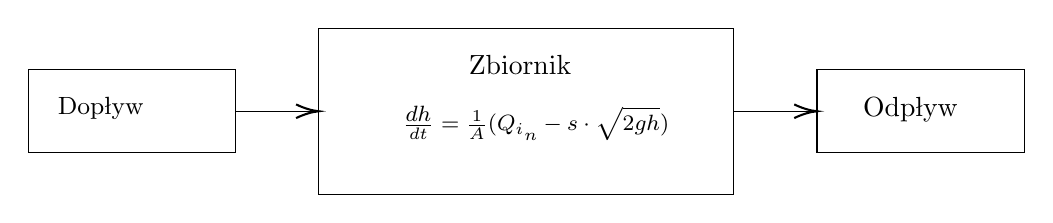
\begin{tikzpicture}[x=0.75pt,y=0.75pt,yscale=-1,xscale=1]

\draw   (110,30) -- (210,30) -- (210,70) -- (110,70) -- cycle ;
\draw   (250,10) -- (450,10) -- (450,90) -- (250,90) -- cycle ;
\draw   (490,30) -- (590,30) -- (590,70) -- (490,70) -- cycle ;
\draw    (210,50) -- (248,50) ;
\draw [shift={(250,50)}, rotate = 180] [color={rgb, 255:red, 0; green, 0; blue, 0 }  ][line width=0.75]    (10.93,-3.29) .. controls (6.95,-1.4) and (3.31,-0.3) .. (0,0) .. controls (3.31,0.3) and (6.95,1.4) .. (10.93,3.29)   ;
\draw    (450,50) -- (488,50) ;
\draw [shift={(490,50)}, rotate = 180] [color={rgb, 255:red, 0; green, 0; blue, 0 }  ][line width=0.75]    (10.93,-3.29) .. controls (6.95,-1.4) and (3.31,-0.3) .. (0,0) .. controls (3.31,0.3) and (6.95,1.4) .. (10.93,3.29)   ;

\draw (123,42) node [anchor=north west][inner sep=0.75pt]  [font=\small] [align=left] {Dopływ};
\draw (321,22) node [anchor=north west][inner sep=0.75pt]   [align=left] {Zbiornik};
\draw (511,42) node [anchor=north west][inner sep=0.75pt]   [align=left] {Odpływ};
\draw (354.5,56) node  [font=\footnotesize]  {${\frac{{\displaystyle dh}}{dt} =\frac{1}{A}( Q_{i}}_{n} -s\cdot \sqrt{2gh} )$};

\end{tikzpicture}
\caption{Schemat obiektu} \label{fig:schemat}
\end{figure}

W celu wyznaczenia odpowiedniej wysokości słupa cieczy napisano algorytm wykorzystujący biblioteki \textit{numpy} oraz \textit{matplotlib}. Program zaprezentowano na listingu \ref{kod}. Można go pobrać z \href{https://github.com/KGrzeg/projekt-zbiornik}{repozytorium Github}.

\lstinputlisting[caption={Kod programu symulacji i animacji},captionpos=b,language=Python,label=kod]{animacja.py}

\begin{figure}[h!]
    \centering
    \includegraphics[scale=0.5]{animacja}
    \caption{Pojedyncza klatka animacji}
    \label{fig:animacja}
\end{figure}

\section{Podsumowanie}
Kod spełnia swoje zadanie animując obiekt zbiornika z wodą, który jest uzupełniany w czasie rzeczywistym. Animacja odzwierciedla ten proces wykorzystując równanie różniczkowe podane w równaniu  \ref{rozniczka} . Cały program funkcjonuje zgodnie z przeznaczeniem, dlatego można wywnioskować, iż zadanie zostało wykonane w sposób \textbf{\textit{poprawny}}. 

\begin{thebibliography}{9}
\bibitem{Symulacja}
mgr inż. Karol Miądlicki, Instytut Technologii Mechanicznej\newline
\textit{Ćwiczenie laboratoryjne nr 1: Symulacja zmian poziomu cieczy w zbiorniku oraz układzie zbiorników.} \newline
Zachodniopomorski Uniwersytet Technologiczny w Szczecinie, 2021.

\bibitem{Matplotlib} 
Parul Pandey: \textit{Animations with Matplotlib},
\\\texttt{https://towardsdatascience.com/animations-with-matplotlib-d96375c5442c}
\end{thebibliography}

\end{document}
